

%-------------------------------------------------------------------------------
% Dokumenten Klasse
\documentclass[
	final,
	a4paper,
	oneside,
	parskip=full,
	headings=standardclasses,
	headings=big,
	pointednumbers
]{scrartcl}

%-------------------------------------------------------------------------------
% Packete nutzen
\usepackage[T1]{fontenc}
\usepackage[utf8]{inputenc}
\usepackage[left=15mm,right=20mm,top=17mm,bottom=17mm,footskip=0.7cm]{geometry}
\usepackage{amsmath}
\usepackage{amssymb}
\usepackage{mathtools}
\usepackage{mathtools}
\usepackage{bm}

%-------------------------------------------------------------------------------
% Andere Schriftart
\usepackage{lmodern}

%-------------------------------------------------------------------------------
% xcolor
\usepackage[svgnames,table]{xcolor}

%-------------------------------------------------------------------------------
% scrlayer-scrpage
\usepackage{scrlayer-scrpage}
\pagestyle{scrheadings}
\clearpairofpagestyles

\cfoot{\pagemark}

%-------------------------------------------------------------------------------
% array
\usepackage{array}
\newcolumntype{A}[1]{>{\raggedright\let\newline\\\arraybackslash\hspace{0pt}}p{#1}}
\newcolumntype{B}[1]{>{\centering\let\newline\\\arraybackslash\hspace{0pt}}p{#1}}
\newcolumntype{C}[1]{>{\raggedleft\let\newline\\\arraybackslash\hspace{0pt}}p{#1}}

\newcolumntype{D}[1]{>{\raggedright\let\newline\\\arraybackslash\hspace{0pt}}m{#1}}
\newcolumntype{E}[1]{>{\centering\let\newline\\\arraybackslash\hspace{0pt}}m{#1}}
\newcolumntype{F}[1]{>{\raggedleft\let\newline\\\arraybackslash\hspace{0pt}}m{#1}}

\newcolumntype{G}[1]{>{\raggedright\let\newline\\\arraybackslash\hspace{0pt}}b{#1}}
\newcolumntype{H}[1]{>{\centering\let\newline\\\arraybackslash\hspace{0pt}}b{#1}}
\newcolumntype{I}[1]{>{\raggedleft\let\newline\\\arraybackslash\hspace{0pt}}b{#1}}


%-------------------------------------------------------------------------------
% tabularx
\usepackage{tabularx}
\usepackage{ltablex}
\usepackage{makecell}

%-------------------------------------------------------------------------------
% TikZ
\usepackage{tikz}
\usetikzlibrary{shapes, positioning, arrows, decorations, calc, fit, intersections}

%-------------------------------------------------------------------------------
% Listings
\usepackage{listings}
\newcommand{\listingMatlab}[2][]{
	\lstset{
		language=Matlab,
		breaklines=true,
		numbers=left,
		numberstyle=\tiny,
		numbersep=5pt,
		captionpos=b,
		basicstyle=\footnotesize\ttfamily,
		stringstyle=\color{magenta},
		identifierstyle=\color{black},
		keywordstyle=\color{blue}, 
		commentstyle=\color{DarkGreen}
	}
	\lstinputlisting[caption={\texttt{\detokenize{#2}}},#1]{#2}
}
\lstnewenvironment{algorithm}[1][] %defines the algorithm listing environment
{
    \lstset{ %this is the stype
        mathescape=true,
        frame=tB,
        numbers=left, 
        numberstyle=\tiny,
        basicstyle=\scriptsize, 
        keywordstyle=\color{black}\bfseries,
        keywords={,input, output, return, datatype, function, in, if, else, foreach, while, begin, end, } 
        numbers=left,
        xleftmargin=.04\textwidth
    }
}
{}


%-------------------------------------------------------------------------------

\RedeclareSectionCommand[
  afterindent=false,
  beforeskip=0.8\baselineskip,
  afterskip=0.4\baselineskip]{section}
\RedeclareSectionCommand[
  afterindent=false,
  beforeskip=0.8\baselineskip,
  afterskip=0.4\baselineskip]{subsection}

%-------------------------------------------------------------------------------
% 

\newcommand{\colouredcircle}{%
    \tikz{
        \useasboundingbox (-0.2em,-0.32em) rectangle(0.2em,0.32em);
        \draw[line width=0.03em] (0,0) circle(0.10em);
    }}



%-------------------------------------------------------------------------------
% enumitem
\usepackage{enumitem}
\newlist{tabenum}{enumerate}{3}
\setlist[tabenum,1]{
    leftmargin=*,
    label=\protect\colouredcircle,
    topsep=0ex,
    partopsep=0ex,
    noitemsep
}
\setlist[tabenum,2]{
    leftmargin=*,
    label=\protect\colouredcircle,
    topsep=0ex,
    partopsep=0ex,
    noitemsep
}
\setlist[tabenum,3]{
    leftmargin=*,
    label=\protect\colouredcircle,
    topsep=0ex,
    partopsep=0ex,
    noitemsep
}

\newcommand{\f}[2]{\frac{#1}{#2}}
\newcommand{\fs}[2]{{\tfrac{#1}{#2}}}

% kl = ()
\newcommand{\kl}[1]{{\left( #1 \right)}}

% kq = {}
\newcommand{\kq}[1]{{\left\{ #1 \right\}}}

% ks = []
\newcommand{\ks}[1]{{\left[ #1 \right]}}

% 
\newcommand{\abs}[1]{{\vert #1 \vert}}


\newcommand{\txb}[1]{{\color{blue}#1}}
\newcommand{\txr}[1]{{\color{red}#1}}
\newcommand{\txo}[1]{{\color{orange}#1}}
\newcommand{\txgr}[1]{{\color{grey}#1}}
\newcommand{\tb}[1]{\textbf{#1}}
\newcommand{\ti}[1]{\textit{#1}}

\newcommand{\tc}[1]{\multicolumn{1}{r|}{#1}}

%-------------------------------------------------------------------------------
% 
\usepackage{xparse}
% 1: Subscription  (default: '')
% 2: Funktion Name (default: 'f')
% 3: Argument      (default: 'x')
% \fx         = f(x)
% \fx[1]      = f_1(x)
% \fx[][u]    = u(x)
% \fx[][u][x] = u(x)
% \fx[][f][u] = f(u)
\NewDocumentCommand{\fx}{ O{} O{f} O{x} }{{#2_{#1}{\left( #3 \right)}}}
\NewDocumentCommand{\dfx}{ O{} O{f} O{x} }{{#2'_{#1}{\left( #3 \right)}}}
\NewDocumentCommand{\dx}{ O{} }{{\Delta x^{#1}}}
\NewDocumentCommand{\dy}{ O{} }{{\Delta y^{#1}}}
\NewDocumentCommand{\dt}{ O{} }{{\Delta t^{#1}}}
\NewDocumentCommand{\du}{ O{} }{{\Delta u^{#1}}}
\NewDocumentCommand{\px}{ O{} }{{\partial x^{#1}}}
\NewDocumentCommand{\py}{ O{} }{{\partial y^{#1}}}
\NewDocumentCommand{\pt}{ O{} }{{\partial t^{#1}}}
\NewDocumentCommand{\pu}{ O{} }{{\partial u^{#1}}}
\NewDocumentCommand{\p}{ O{} }{{\partial^{#1}}}
\NewDocumentCommand{\re}{ O{} }{{\mathbb{R}^{#1}}}

\NewDocumentCommand{\xyz}{ O{x} O{y} O{z} }{#1 #2 #3}
% 1: Value
% 2: Key
% 3: Background Color
\NewDocumentCommand{\tfill}{ O{} O{} O{blue!20} }{%
    \tikz[baseline, every node/.style={inner sep=3pt,outer sep=0pt,minimum width=3mm,minimum height=4mm}]{
        \node[fill=#3,anchor=base] (#2) {#1};
    }
}
\NewDocumentCommand{\tfillc}{ O{} O{} }{%
    \tikz[baseline, every node/.style={inner sep=2pt,outer sep=0pt}]{
        \node[fill=#2,anchor=base] {#1};
    }
}

\NewDocumentCommand{\tdrawc}{ O{} O{} }{%
    \tikz[baseline, every node/.style={inner sep=2pt,outer sep=0pt}]{
        \node[rectangle,draw=#2,anchor=base] {#1};
    }
}

\NewDocumentCommand{\tcrossc}{ O{} O{} }{%
    \tikz[baseline, every node/.style={inner sep=0pt,outer sep=0pt}]{
        \node[draw=#2,anchor=base,cross out,line width=1pt] {#1};
    }
}

\newcommand{\tfillb}[1]{\tfillc[#1][blue!20]}
\newcommand{\tfillo}[1]{\tfillc[#1][orange!40]}
\newcommand{\tfillg}[1]{\tfillc[#1][Green!20]}
\newcommand{\tfilly}[1]{\tfillc[#1][yellow!40]}
\newcommand{\tfillr}[1]{\tfillc[#1][red!20]}
\newcommand{\tfillv}[1]{\tfillc[#1][Violet!20]}
\newcommand{\tfillt}[1]{\tfillc[#1][Turquoise!20]}
\newcommand{\tfillgr}[1]{\tfillc[#1][Gray!20]}


\newcommand{\tdrawb}[1]{\tdrawc[#1][blue!40]}
\newcommand{\tdrawo}[1]{\tdrawc[#1][orange!60]}
\newcommand{\tdrawg}[1]{\tdrawc[#1][Green!40]}
\newcommand{\tdrawy}[1]{\tdrawc[#1][yellow!60]}
\newcommand{\tdrawr}[1]{\tdrawc[#1][red!40]}
\newcommand{\tdrawv}[1]{\tdrawc[#1][Violet!40]}
\newcommand{\tdrawt}[1]{\tdrawc[#1][Turquoise!40]}
\newcommand{\tdrawgr}[1]{\tdrawc[#1][Gray!40]}
\newcommand{\tdrawk}[1]{\tdrawc[#1][black]}


\newcommand{\tcrossr}[1]{\tcrossc[#1][red]}
\newcommand{\tcrossg}[1]{\tcrossc[#1][green]}
\newcommand{\tcrossb}[1]{\tcrossc[#1][blue]}

\begin{document}
    \section*{StatQuest: Decision Tree}
    
        StatQuest is growing up, StatQuest is growing down.
        
        Here's a simple decision tree
        
        If a person loves StatQuest theme songs...
        Then that person is awesome!
        
        And if a person does not love StatQuest theme songs...
        Then that person is slightly less than awesome.
        
        In general, a decision tree asks a question...
        ... and classifies the person based on the answer.
        It's no big deal!
        This decision tree is based on a "yes/no" question...
        ... but it is just as easy to build a tree from numeric data.
        
        If a person has a really high resting heart rate...
        ... then that person had better see a doctor.
        And if a person does not have a super high resting heart rate...
        then that person is doing OK.
        
        Here's one more simple decision tree.
        This decision tree is based on ranked data, where
        1 is super hungry and
        2 is moderately hungry.
        If a person is super hungry, they need to eat.
        And if a person is moderately hungry, they just need a snack.
        And if they are not hungry at all, then there's no need to eat.
        Note: the classification can be categories or numeric.
        
        In this case, we are using mouse weight...
        ... to predict mouse size.
        
        Here's a more complicated decision tree...
        It combines numeric data with yes/no data.
        Notice that the cutoff for resting heart rate isn't always the same.
        In this case, its 100bpm on the left side and 120bpm on the right side.
        And the order of questions on the left side,
        first about resting heart rate then about eating donuts doesn't
        have to be the same on the right side. On the right side, the question about
        donuts is asked first.
        Lastly, the final classification can be repeated.
        For the most part, decision trees are pretty intuitive to work with.
        You start at the top... and work your way down... and down...
        till you get to a point, where you can't go any further.
        And that's how you classify a sample.
        
        Oh no, Jargon Alert!
        
        The very top of the tree is called the "Root Node" or just "The Root".
        These are called "Internal Nodes", or just "Nodes".
        Internal Nodes have arrows pointing to them...
        ... and they have arrows pointing away from them.
        Lastly, these are called "Leaf Nodes", or just "Leaves".
        Leaf Nodes have arrows pointing to them...
        ... but there are no arrows pointing away from them.
        
        Now we are ready to talk about how to go from a raw table of data...
        ... to a decision tree!
        
        In this example, we want to create a tree that uses chest pain (Schmerzen in der Brust),
        good blood circulation and blocked artery status to predict...
        ... whether or not a patient has heart disease.
        The first thing we want to know is whether Chest Pain,
        Good Blood Circulation or Blocked Arteries should be at the
        very top of our tree.
        We start by looking at how well Chest Pain alone predicts heart disease...
        
        Here's a little tree that only takes chest pain into account.
        The first patient does not have chest pain and does not have heart disease.
        And we keep track of that here.
        The 2nd patient has chest pain and heart disease.
        And we keep track of that here.
        The 3rd patient has chest pain but does not have heart disease.
        The 4th patient has chest pain and heart disease.
        Ultimately, we look at chest pain and heart disease for all 303
        patients in this study.
        Now we do the exact same thing for Good Blood Circulation.
        Lastly, we look at how Blocked Arteries separates the patients with
        and without heart disease.
        Since we don't know if this patient had blocked arteries or not,
        we'll skip it.
        However, there are alternatives that I'll discuss in a follow up video.
        Remember, the goal is to decide whether Chest Pain,
        Good Blood Circulation or Blocked Arteries should be the first thing
        in our decision tree (aka The Root Node.
        So we looked at how well Chest Pain separated patients with and without
        heart disease.
        It did OK, but wasn't perfect.
        Most of the patients with heart disease ended up in this leaf node...
        ... and most of the patients without heart disease ended up in this leaf node.
        Then we looked at how well Good Blood Circulation separated patients with
        and without heart disease.
        It wasn't perfect either.
        Lastly, we looked at how well Blocked Arteries separated patients
        with and without heart disease.
        Note. The total number of patients with heart disease is different
        from Chest Pain,
        Good Blood Circulation and Blocked Arteries because some patients
        had measurements for Chest Pain, but not for Blocked Arteries, etc.
        Oh no, it's another one of those ghastly jargon alerts.
        Because none of the leaf nodes are 100% "YES Heart Disease" or
        "NO Heart Disease", they are all considered "impure" (unrein, schmutzig).
        To determine which separation is best, we need a way to measure and
        compare "impurity".
        There are a bunch of ways to measure impurity, but I'm just going to
        focus on a very popular one called "Gini".
        To be honest, I don't know why it's called Gini.
        I looked around on the internet and couldn't find anything.
        However, if you know, please put it in the comments below.
        I would love to know!
        
        Regardless, the good news is calculating Gini impurity is easy.
        Let's start by calculating Gini impurity for Chest Pain...
        For this leaf, the Gini impurity equals

        $1 - (the probability of "yes")^2 [squared] - (the probability of "no")^2$

        Now lets plug in some numbers:
        
        the probability of yes equals 105 divided by the total number of people
        in this leaf node. And the probability of no equals 39 divided by the total
        number of people in this leaf node. After we've done the math, we get 0.395.
        That is to say: the Gini impurity for the leaf node on the left equals 0.395.
        Now let's calculate the Gini impurity for this leaf node on the right...
        Just like before it equals
        $1 - (the probability of "yes")^2 [squared] - (the probability of "no")^2$

        And the probability of yes is 34 divided by the total number of people in
        this leaf node. And the probability of no equals 125 divided 
        by the total number of people in this leaf node.
        And if we do the math, we get 0.336.
        Now that we have measured the Gini impurity for both leaf nodes,
        we can calculate the total Gini impurity for using Chest Pain
        to separate patients with and without heart disease.
        Because this leaf node represents 144 patients...
        ...and this leaf node represents 159 patients...
        ... the leaf nodes do not represent the same number of patients.
        Thus, the total Gini impurity for using Chest Pain to separate patients
        with and without heart disease is the weighted average of the leaf
        node impurities.
        
        So to calculate the weighted average, we take the total number of
        people in the left leaf node and divide by the total number of people
        in both leaf nodes. We then multiply that fraction by the Gini impurity
        for the left leaf node, then we take the total number of people in the
        right leaf node divided by the total number of people in both leaf nodes
        and then mutiply that fraction by the Gini impurity for the right leaf
        node.

        $144 / (144+159) * 0.395 + 159 / (144+15) * 0.336$

        After we do the math, we get 0.364. Thus, the total
        Gini impurity for Chest Pain equals 0.364. And since I'm
        such a nice guy, I'm going to cut to the chase (auf den Punkt bringen)
        and tell you that the Gini impurity for good blood circulation equals 
        0.360 and the Gini impurity for Blocked Arteries equals 0.381
        
        Good blood circulation has the lowest impurity. It separates patients
        with and without heart disease the best.
        So we will use it at the root of the tree.
        Note: When we divided all of the patients using Good Blood Circulation,
        we ended up with "impure" leaf nodes.
        That is to say, each leaf contains a mixture of patients with and without
        Heart Disease.
        That means, the 164 patients with and without heart disease that ended up
        in this leaf node...
        ... are now in this node in the tree...
        ... and the 133 patients with and without heart disease that ended
        up in this leaf node...
        ... are now in this node in the tree.
        Now we need to figure how well Chest Pain and Blocked Artieries separate
        these 164 patients (37 with heart disease and 127 without heart disease).
        Just like we did before, we separate these patients based on Chest Pain
        and then calculate the Gini impurity value. In this case it's 0.3.
        And then we do the exact same thing for blocked artieries.
        Since blocked artieries has the lowest Gini impurity, we will use it
        at this node to separate patients.
        Here's the tree that we've worked out so far.
        We started at the top by separating patients with Good Circulation...
        ... then we used Blocked Arteries to separate patients on the left side
        of the tree.
        All we have left is Chest Pain, so first we'll see how well it separates
        these 49 patients (24 with heart disease and 25 without heart disease).
        Nice! Chest pain does a good job separating the patients...
        ... so these are the final leaf nodes on this branch of the tree.
        Now let's see what happens when we use chest pain to divide these 115
        patients (13 with heart disease and 102 without).
        Note. The vast majority of the patients in this node (89%) don't
        have heart disease.
        Here's how chest pain divides these patients.
        Do these new leaves separate patients better than what we had before?
        Well, let's calculate the Gini impurity for it. In this case, it's 0.29.
        The Gini impurity for this node before using chest pain to separate
        patients is 0.2.
        The impurity is lower if we don't separate patients using Chest pain.
        So we will make it a leaf node.
        OK, at this point we've worked out the entire left side of the tree...
        ... now we need to work out the right side of the tree...
        The good news is that we follow the exact same steps as we did on the
        left side:
        1) First, we calculate all the Gini impurity scores
        2) Second, if the node ifself has the lowest score, than
        there is no point in separating the patients any more and it become
        a leaf node.
        3) Third, if separating the data results in an improvement, than
        pick the separation with the lowest impurity value.
        
        Hooray!! We made a decision tree!
        
        So far we've seen how to build a tree with "yes/no" questions at each step...
        ... but what if we have numeric data, like patient weight?
        Imagine if this were our data...
        How do we determine what's the best weight to use to divide the patients?
        Step 1) Sort the patients by weight, lowest to highest.
        Step 2) Calculate the average weight for all adjacent patients.
        Step 3) Calculate the impurity values for each average weight.
        For example, we can calculate the impurity value for weights less than < 167.5
        ... dooba ... Ultimately, we get 0.3 as the impurity value for this weight.
        And then we calculate the impurity values for the other weights as well.
        The lowest impurity occures when we separate using weight less than < 205
        ... so this is the cutoff and impurity value we will use when we compare
        weight to Chest Pain or Blocked Arteries.
        Now we've seen how to builda tree with...
        1) "yes/no" questions at each step...
        2) Numeric data, like patient weight...
        Now let's talk about ranked data, like "rank my jokes on a scale of
        1 to 4", and multiple choice data, like "which color do you like, red,
        blue or green?"
        
        Ranked data is similar to numeric data, except instead now we calculate
        impurity scores for all of the possible ranks.
        So if people could rank my jokes from 1 to 4 (4 being the funniest),
        we could calculate the following impurity scores...
        Joke Rank less than or equal to <= 1
        Joke Rank less than or equal to <= 2
        and Joke Rank less than or equal to <= 3
        Note. We don't have to calculate an impurity score for Joke Rang <= 4
        because that would include everyone.
        
        When there are multiple choices, like "color choice can be blue, green or
        red", you calculate an impurity score for each one as well as each possible
        combination.
        For this example, with three colors (blue, green and red) we get
        the following options.
        1) Color choice: blue
        2) Color choice: green
        3) Color choice: red
        4) Color choice: blue or green
        5) Color choice: blue or red
        And lastly
        6) Color choice: green or red
        Note. we don't have to calculate an impurity score for
        "Color Choice: Blue or Green or Red" since that includes everyone.
        
        BAM!! Now we know how to make and use decision trees!
        Tune in next time for random forest... that's when the fun really begins!



    \begin{center}
        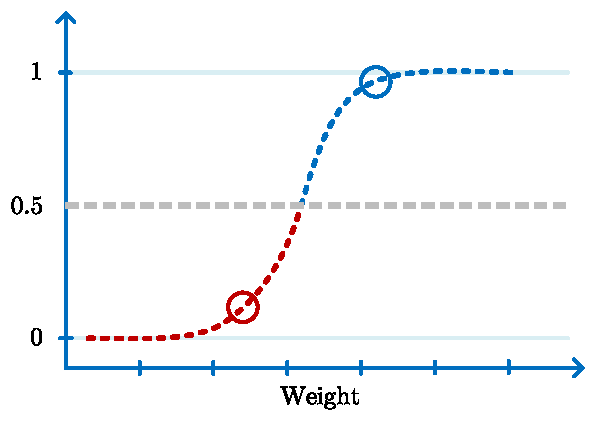
\includegraphics[height=5cm]{StatQuest_ROC_and_AUC_Obese_Threshold.pdf}
    \end{center}



    

\end{document}